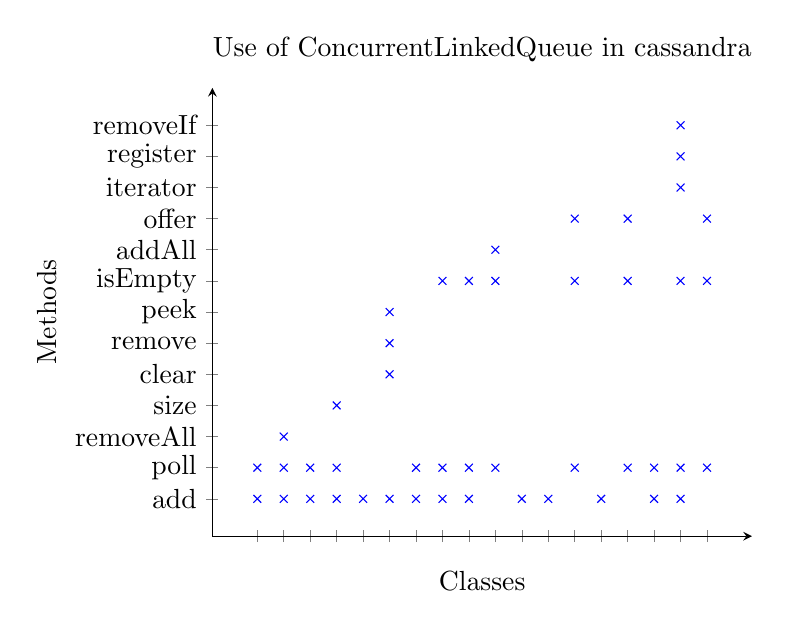
\begin{tikzpicture}
\begin{axis}[scatter/classes={U={mark=+,red}, NU={mark=x,blue}}, legend pos=outer north east,axis x line=bottom, axis y line=left, enlarge x limits=true, xlabel = {Classes}, ylabel = {Methods}, enlarge y limits=true, xtick = data, xticklabels = {,,},ytick=data, yticklabels={add,poll,removeAll,size,clear,remove,peek,isEmpty,addAll,offer,iterator,register,removeIf}, title={Use of ConcurrentLinkedQueue in cassandra}]
\addplot[scatter,only marks, scatter src=explicit symbolic]
coordinates {
(0,0) [NU]
(0,1) [NU]
(1,0) [NU]
(1,2) [NU]
(1,1) [NU]
(2,0) [NU]
(2,1) [NU]
(3,0) [NU]
(3,3) [NU]
(3,1) [NU]
(4,0) [NU]
(5,0) [NU]
(5,4) [NU]
(5,5) [NU]
(5,6) [NU]
(6,0) [NU]
(6,1) [NU]
(7,0) [NU]
(7,7) [NU]
(7,1) [NU]
(8,0) [NU]
(8,7) [NU]
(8,1) [NU]
(9,8) [NU]
(9,7) [NU]
(9,1) [NU]
(10,0) [NU]
(11,0) [NU]
(12,9) [NU]
(12,7) [NU]
(12,1) [NU]
(13,0) [NU]
(14,9) [NU]
(14,7) [NU]
(14,1) [NU]
(15,0) [NU]
(15,1) [NU]
(16,0) [NU]
(16,10) [NU]
(16,7) [NU]
(16,1) [NU]
(16,11) [NU]
(16,12) [NU]
(17,9) [NU]
(17,7) [NU]
(17,1) [NU]
};
\end{axis}
\end{tikzpicture}